\documentclass[a4paper,10pt]{article}
\usepackage[dvips]{color,graphicx}
\usepackage[dvips, bookmarks, colorlinks=false]{hyperref}

%opening
\title{Math650 Homework 7}
\author{Yu Huang}
\date{2006-10-12}
\begin{document}

\maketitle

\section{Question 1}
Prove that the least square estimates of $\beta$ and $\sigma^2$ are also the MLE estimates.
\begin{eqnarray}
L(\beta, \sigma^2|x) = (2\pi\sigma^2)^{-n/2}exp(-\frac{\|Y-X\| ^2}{2\sigma^2}) \nonumber \\
l(\beta, \sigma^2|x) = log(L(\beta, \sigma^2|x)) = -\frac{n}{2}log(2\pi) - \frac{n}{2}log(\sigma^2) - \frac{1}{2\sigma^2}\|Y-X\| ^2 \nonumber
\end{eqnarray}

Now let
\begin{eqnarray}
\frac{\partial{l}}{\partial{\beta}} = -\frac{1}{2\sigma^2}(-2X^T Y+2X^TX\beta)=0 \nonumber
\end{eqnarray}

This is due to
\begin{eqnarray}
\frac{\partial{\beta^TA}}{\partial{\beta}} = A \nonumber \\
\frac{\partial{\beta^TA\beta}}{\partial{\beta}} = 2A\beta \nonumber
\end{eqnarray}

We can get
\begin{eqnarray}
\hat{\beta} = (X^TX)^{-1}X^TY
\end{eqnarray}

Now put $\hat{\beta}$ into the likelihood function and let
\begin{eqnarray}
\nu = \sigma^2 \nonumber \\
\frac{\partial{l}}{\partial{\nu}} = -\frac{n}{2\nu} + 1/2\nu^{-2}\|Y-X\hat{\beta}\|^2 = 0 \nonumber
\end{eqnarray}

We can get
\begin{eqnarray} \label{eq:2}
\nu = \frac{\|Y-X\hat{\beta}\|^2}{n} = \frac{1}{n}Y^T(I-X(X^TX)^{-1}X^T)Y
\end{eqnarray}

The last equality in (\ref{eq:2}) is due to the fact that $P=X(X^TX)^{-1}X^T$ (and $I-P$) are iden-potent matrices.

\section{Question 2}
Check the example of Scottish hill races in Chapter 6 of Venables and Ripley. The influential points are one labeled in figure~\ref{f1}. Codes are appended~\ref{appendix1}

\begin{figure}
\includegraphics[angle=-90, width=1\textwidth]{figures/math650_hw7_fig1.eps}
\caption{Influential points in question 2}\label{f1}
\end{figure}

\section{Question 3}
\subsection{Scatterplot after log-transformation}
Take the logit transformation of proportion unremoved ($p$), $LOGIT=log[p/(1-p)]$. Take the log of the duration. After these two transformations, a scatter plot is shown~\ref{f2}. Both QUEEN and WORKER show a linear trend. The question is how related these two linear trends are. 

\subsection{Linear regression with interaction term}
The formula is $LOGIT~LOGDURATION+BEE+LOGDURATION*BEE$. The residual, QQ plots and et al. are in figure~\ref{f3}. The linear regression summary is
\begin{verbatim}
Call:
lm(formula = LOGIT ~ LOGDURATION + BEE + LOGDURATION * BEE, data = data)

Residuals:
     Min       1Q   Median       3Q      Max
-1.29598 -0.57195 -0.07547  0.24682  5.00989

Coefficients:
                      Estimate Std. Error t value Pr(>|t|)
(Intercept)            -0.5813     0.7733  -0.752    0.456
LOGDURATION             0.5773     0.2876   2.008    0.051 .
BEEWORKER              -0.4776     1.3186  -0.362    0.719
LOGDURATION:BEEWORKER   0.6067     0.4259   1.425    0.161
---
Signif. codes:  0 '***' 0.001 '**' 0.01 '*' 0.05 '.' 0.1 ' ' 1

Residual standard error: 0.9865 on 43 degrees of freedom
Multiple R-Squared: 0.5422,     Adjusted R-squared: 0.5102
F-statistic: 16.97 on 3 and 43 DF,  p-value: 2.024e-07
\end{verbatim}

Figure~\ref{f4} is the regression lines out of the parallel line model.

Here two problems arise.
\begin{enumerate}
 \item Normal Q-Q, Residuals vs Leverage, Residuals vs fitted, all these plots show that data No. 41 is an outlier.
 \item P-value for the coefficients of BEEWORKER and LOGDURATION:BEEWORKER are not significant. This suggests one of them is redundant. The interaction term has higher suspicion.
\end{enumerate}
We are gonna tackle these two problems one by one.

\subsection{Linear regression with interaction after removal of outlier}
Here we removed the outlier and applied the procedure above. The residual, QQ plots and et al. are in figure~\ref{f5}. Here's the summary report.
\begin{verbatim}
Call:
lm(formula = LOGIT ~ LOGDURATION + BEE + LOGDURATION * BEE, data = data)

Residuals:
     Min       1Q   Median       3Q      Max
-0.93491 -0.44372 -0.05707  0.32178  1.35129

Coefficients:
                      Estimate Std. Error t value Pr(>|t|)
(Intercept)            -0.5813     0.4577  -1.270  0.21111
LOGDURATION             0.5773     0.1702   3.392  0.00152 **
BEEWORKER              -0.5350     0.7805  -0.685  0.49684
LOGDURATION:BEEWORKER   0.4845     0.2524   1.919  0.06175 .
---
Signif. codes:  0 '***' 0.001 '**' 0.01 '*' 0.05 '.' 0.1 ' ' 1

Residual standard error: 0.5839 on 42 degrees of freedom
Multiple R-Squared: 0.6879,     Adjusted R-squared: 0.6656
F-statistic: 30.86 on 3 and 42 DF,  p-value: 1.057e-10
\end{verbatim}
Figure~\ref{f6} is the regression lines out of the parallel line model.

This time, no outlier appeared and P-values get more significant. But the redundancy problem of BEEWORKER and LOGDURATION:BEEWORKER is still there.

\subsection{Linear regression WITHOUT interaction after removal of outlier}
So we did linear regression without interaction. The residual, QQ plots and et al. are in figure~\ref{f7}. Here's the summary report.
\begin{verbatim}
Call:
lm(formula = LOGIT ~ LOGDURATION + BEE, data = data)

Residuals:
     Min       1Q   Median       3Q      Max
-1.13897 -0.42493 -0.05872  0.32673  1.33321

Coefficients:
            Estimate Std. Error t value Pr(>|t|)
(Intercept)  -1.1597     0.3551  -3.266 0.002147 **
LOGDURATION   0.7976     0.1296   6.156 2.17e-07 ***
BEEWORKER     0.9041     0.2235   4.045 0.000214 ***
---
Signif. codes:  0 '***' 0.001 '**' 0.01 '*' 0.05 '.' 0.1 ' ' 1

Residual standard error: 0.6019 on 43 degrees of freedom
Multiple R-Squared: 0.6605,     Adjusted R-squared: 0.6447
F-statistic: 41.84 on 2 and 43 DF,  p-value: 8.166e-11
\end{verbatim}
Figure~\ref{f8} is the regression lines out of the parallel line model.

All right, now everything is good. P-values are significant and no outlier. So this simpler parallel line model is actually what we need. As we see, the trends between LOGIT and LOGDURATION are similar for both QUEEN and WORKER. If we interpret our linear model by going back to the data without log-transformation, we'll find WORKER is $exp(-1.1597)*exp(0.9041)$ times more efficient than QUEEN.


\begin{figure}
\includegraphics[angle=-90, width=1\textwidth]{figures/math650_hw7_fig2.eps}
\caption{Scatterplot of LOGIT vs LOGDURATION}\label{f2}
\end{figure}
\begin{figure}
\includegraphics[angle=-90, width=1\textwidth]{figures/math650_hw7_fig3.eps}
\caption{Linear regression plots with interaction and full data}\label{f3}
\end{figure}
\begin{figure}
\includegraphics[angle=-90, width=1\textwidth]{figures/math650_hw7_fig4.eps}
\caption{Regression line, black is QUEEN, red is WORKER}\label{f4}
\end{figure}
\begin{figure}
\includegraphics[angle=-90, width=1\textwidth]{figures/math650_hw7_fig5.eps}
\caption{Linear regression plots with interaction and removel of data No.41}\label{f5}
\end{figure}
\begin{figure}
\includegraphics[angle=-90, width=1\textwidth]{figures/math650_hw7_fig6.eps}
\caption{Regression line, black is QUEEN, red is WORKER, outlier removed}\label{f6}
\end{figure}
\begin{figure}
\includegraphics[angle=-90, width=1\textwidth]{figures/math650_hw7_fig7.eps}
\caption{Linear regression plots without interaction and removel of data No.41}\label{f7}
\end{figure}
\begin{figure}
\includegraphics[angle=-90, width=1\textwidth]{figures/math650_hw7_fig8.eps}
\caption{Regression line, black is QUEEN, red is WORKER, outlier removed, no interaction}\label{f8}
\end{figure}

\section{Appendix I}
\label{appendix1}
\begin{verbatim}
library(MASS)
hills.lm  = lm(time~dist+climb, data=hills)

#frame(); par(fig=c(0, 0.6, 0, 0.55))
postscript('~/script/test/math650/figures/math650_hw7_fig1.eps')
hills.fitted = fitted(hills.lm)
hills.studres = studres(hills.lm)
plot(hills.fitted, hills.studres, xlim=c(0,200), ylim=c(-2,8))
abline(h=0, lty=2)
#label the influential points
text(hills.fitted[18], hills.studres[18], row.names(hills[18,]), pos=4)
text(hills.fitted[7], hills.studres[7], row.names(hills[7,]), pos=4)
#identify(hills.fitted, hills.studres, row.names(hills))
dev.off()
\end{verbatim}

\section{Appendix II}
\label{appendix2}
\begin{verbatim}
#chap_11_no_10
library(lattice)
data1 = read.csv("/usr/local/doc/statistical_sleuth/ASCII/ex0328.csv")
LOGIT = data1$REMOVED/(1-data1$REMOVED)
LOGDURATION = log(data1$DURATION)
data2 = cbind(data1, LOGIT, LOGDURATION)
histogram(~LOGIT|BEE, data=data2)
histogram(~LOGDURATION|BEE, data=data2)

postscript('~/script/test/math650/figures/math650_hw7_fig2.eps')
xyplot(LOGIT~LOGDURATION|BEE, data=data2)
dev.off()

linear_model_interaction = function(data, fig_fname)
{
reg = lm(LOGIT~LOGDURATION+BEE+LOGDURATION*BEE, data=data)
print(summary(reg))
postscript(fig_fname)
opar <- par(mfrow = c(2,2), oma = c(0, 0, 1.1, 0))
plot(reg)
par(opar)
dev.off()
return(reg)
}

draw_data_interaction = function(reg, data)
{
intercept_1 = coef(reg)[1]
slope_1 = coef(reg)[2]
intercept_2 = coef(reg)[1] + coef(reg)[3]
slope_2 = coef(reg)[2]+coef(reg)[4]
xyplot(LOGIT~LOGDURATION, data=data, panel=function(x,y,subscripts){
  one <- data[subscripts,]$BEE=="QUEEN"
  two <- data[subscripts,]$BEE=="WORKER"
  lpoints(x[one], y[one], col = 1)
  lpoints(x[two], y[two], col = 2)
  panel.abline(c(intercept_1, slope_1), col=1)
  panel.abline(c(intercept_2, slope_2), col=2)
  }
)
}

reg = linear_model_interaction(data2, '~/script/test/math650/figures/math650_hw7_fig3.eps')
#2006-10-12, very weird, trellis.device() can't be run within draw_data(). It'll give null graphic output.

trellis.device(postscript, color=T, file='~/script/test/math650/figures/math650_hw7_fig4.eps')
draw_data_interaction(reg, data2)
dev.off()

#remove outlier #41
reg = linear_model_interaction(data2[-41,], '~/script/test/math650/figures/math650_hw7_fig5.eps')
#2006-10-12, very weird, trellis.device() can't be run within draw_data(). It'll give null graphic output.

trellis.device(postscript, color=T, file='~/script/test/math650/figures/math650_hw7_fig6.eps')
draw_data_interaction(reg, data2[-41,])
dev.off()

linear_model_no_intr = function(data, fig_fname)
{
reg = lm(LOGIT~LOGDURATION+BEE, data=data)
print(summary(reg))
postscript(fig_fname)
opar <- par(mfrow = c(2,2), oma = c(0, 0, 1.1, 0))
plot(reg)
par(opar)
dev.off()
return(reg)
}

draw_data_no_intr = function(reg, data)
{
intercept_1 = coef(reg)[1]
slope_1 = coef(reg)[2]
intercept_2 = coef(reg)[1] + coef(reg)[3]
slope_2 = coef(reg)[2]
xyplot(LOGIT~LOGDURATION, data=data, panel=function(x,y,subscripts){
  one <- data[subscripts,]$BEE=="QUEEN"
  two <- data[subscripts,]$BEE=="WORKER"
  lpoints(x[one], y[one], col = 1)
  lpoints(x[two], y[two], col = 2)
  panel.abline(c(intercept_1, slope_1), col=1)
  panel.abline(c(intercept_2, slope_2), col=2)
  }
)
}
#remove outlier #41
reg = linear_model_no_intr(data2[-41,], '~/script/test/math650/figures/math650_hw7_fig7.eps')
#2006-10-12, very weird, trellis.device() can't be run within draw_data(). It'll give null graphic output.

trellis.device(postscript, color=T, file='~/script/test/math650/figures/math650_hw7_fig8.eps')
draw_data_no_intr(reg, data2[-41,])
dev.off()
\end{verbatim}

\end{document}
